\documentclass[12pt,a4paper]{article}

%\pdfoutput=1

\usepackage[utf8]{inputenc}
\usepackage[T1]{fontenc}
\usepackage[english]{babel}
\usepackage{amsmath}
\usepackage{mathabx}
\usepackage{lmodern}
\usepackage{listings}
\usepackage{units}
\usepackage{siunitx}
\usepackage{icomma}
\usepackage{graphicx}
\usepackage{caption}
\usepackage{subcaption}
\usepackage{color}
\usepackage{pgf}
\DeclareMathOperator{\acosh}{arccosh}
\newcommand{\N}{\ensuremath{\mathbbm{N}}}
\newcommand{\Z}{\ensuremath{\mathbbm{Z}}}
\newcommand{\Q}{\ensuremath{\mathbbm{Q}}}
\newcommand{\R}{\ensuremath{\mathbbm{R}}}
\newcommand{\C}{\ensuremath{\mathbbm{C}}}
\newcommand{\rd}{\ensuremath{\mathrm{d}}}
\newcommand{\id}{\ensuremath{\,\rd}}
\usepackage{hyperref}
%\usepackage{a4wide} % puts the page numbering further down the page.
\usepackage{pdfpages}
\usepackage{epstopdf}
\DeclareGraphicsExtensions{.eps}
\def\changemargin#1#2{\list{}{\rightmargin#2\leftmargin#1}\item[]}
\let\endchangemargin=\endlist

\title{Handin 2}
\author{Marcus Malmquist, marmalm}
\date{\today}

\begin{document}
\maketitle

\section{Task 1}\label{sec:1}
The $\SI{3}{\deci\bel}$ bandwidth of the signal is approximately $\SI{200}{\hertz}$ from Figure~\ref{fig:task1_ut}.
\begin{figure}[ht!]
  \centering
  \noindent\makebox[\textwidth]{\scalebox{0.90}{% Title: gl2ps_renderer figure
% Creator: GL2PS 1.3.9, (C) 1999-2015 C. Geuzaine
% For: Octave
% CreationDate: Mon May 15 17:24:31 2017
\setlength{\unitlength}{1pt}
\begin{picture}(0,0)
\includegraphics{figures/task1-inc.pdf}
\end{picture}%
\begin{picture}(576,432)(0,0)
\fontsize{10}{0}
\selectfont\put(74.88,42.5189){\makebox(0,0)[t]{\textcolor[rgb]{0.15,0.15,0.15}{{-200}}}}
\fontsize{10}{0}
\selectfont\put(186.48,42.5189){\makebox(0,0)[t]{\textcolor[rgb]{0.15,0.15,0.15}{{-100}}}}
\fontsize{10}{0}
\selectfont\put(298.08,42.5189){\makebox(0,0)[t]{\textcolor[rgb]{0.15,0.15,0.15}{{0}}}}
\fontsize{10}{0}
\selectfont\put(409.68,42.5189){\makebox(0,0)[t]{\textcolor[rgb]{0.15,0.15,0.15}{{100}}}}
\fontsize{10}{0}
\selectfont\put(521.28,42.5189){\makebox(0,0)[t]{\textcolor[rgb]{0.15,0.15,0.15}{{200}}}}
\fontsize{10}{0}
\selectfont\put(69.8755,47.52){\makebox(0,0)[r]{\textcolor[rgb]{0.15,0.15,0.15}{{100000}}}}
\fontsize{10}{0}
\selectfont\put(69.8755,97.8171){\makebox(0,0)[r]{\textcolor[rgb]{0.15,0.15,0.15}{{150000}}}}
\fontsize{10}{0}
\selectfont\put(69.8755,148.114){\makebox(0,0)[r]{\textcolor[rgb]{0.15,0.15,0.15}{{200000}}}}
\fontsize{10}{0}
\selectfont\put(69.8755,198.411){\makebox(0,0)[r]{\textcolor[rgb]{0.15,0.15,0.15}{{250000}}}}
\fontsize{10}{0}
\selectfont\put(69.8755,248.709){\makebox(0,0)[r]{\textcolor[rgb]{0.15,0.15,0.15}{{300000}}}}
\fontsize{10}{0}
\selectfont\put(69.8755,299.006){\makebox(0,0)[r]{\textcolor[rgb]{0.15,0.15,0.15}{{350000}}}}
\fontsize{10}{0}
\selectfont\put(69.8755,349.303){\makebox(0,0)[r]{\textcolor[rgb]{0.15,0.15,0.15}{{400000}}}}
\fontsize{10}{0}
\selectfont\put(69.8755,399.6){\makebox(0,0)[r]{\textcolor[rgb]{0.15,0.15,0.15}{{450000}}}}
\fontsize{11}{0}
\selectfont\put(298.08,31.5188){\makebox(0,0)[t]{\textcolor[rgb]{0.15,0.15,0.15}{{Frequency (Hz)}}}}
\fontsize{11}{0}
\selectfont\put(29.8755,223.56){\rotatebox{90}{\makebox(0,0)[b]{\textcolor[rgb]{0.15,0.15,0.15}{{Power}}}}}
\fontsize{11}{0}
\selectfont\put(298.08,409.6){\makebox(0,0)[b]{\textcolor[rgb]{0,0,0}{{Power Spectral Density of azimuth spectrum}}}}
\end{picture}
}}
  \caption{The spectrum plot of the average along the major axis of the fft of the minor axes.}
  \label{fig:task1_ut}
\end{figure}

\subsection{a}
Using (\ref{eq:resolution_b}) the resolution is $\SI{660}{\milli\metre}$.
\begin{equation}
  \label{eq:resolution_b}
  \Delta x = \frac{v}{B}
\end{equation}

\subsection{b}
Using (\ref{eq:resolution_a}) the resolution is $\SI{650}{\milli\metre}$.
\begin{equation}
  \label{eq:resolution_a}
  \Delta x = \frac{D_a}{2}
\end{equation}

\subsection{c}
When the antenna size decreases the gain will increase and we may have to increase the frequency which can lead to atmospheric attenuation depending on what frequency we choose.
Ultimately the resolution will be limited by the wavelength.

\section{Task 2}
Since $\Theta_a=\SI{3}{\degree}$ we can apprximate $\sin(\Theta_a)\approx\Theta_a$.
Assuming $R_{0,\text{near}}$ is defined in the centering of the cell, the distance to the furthest cell would because $R_{0,\text{far}}=R_{0,\text{near}}+349\Delta R$.

Using (\ref{eq:rangeres}) the synthetic aperture length, $L$, would be $\SI{620}{\metre}$.
\begin{equation}
  \label{eq:rangeres}
  L = R_{0,\text{far}}\Theta_a= (R_{0,\text{near}}+349\Delta R)\Theta_a
\end{equation}
The synthetic aperture length in terms of pixels is $1442$.

\section{Task 3}
\begin{figure}[ht!]
  \centering
  \noindent\makebox[\textwidth]{\scalebox{0.90}{% Title: gl2ps_renderer figure
% Creator: GL2PS 1.3.9, (C) 1999-2015 C. Geuzaine
% For: Octave
% CreationDate: Wed May 24 14:53:39 2017
\setlength{\unitlength}{1pt}
\begin{picture}(0,0)
\includegraphics{figures/task3-inc.pdf}
\end{picture}%
\begin{picture}(576,432)(0,0)
\fontsize{10}{0}
\selectfont\put(74.88,42.5189){\makebox(0,0)[t]{\textcolor[rgb]{0.15,0.15,0.15}{{0}}}}
\fontsize{10}{0}
\selectfont\put(164.16,42.5189){\makebox(0,0)[t]{\textcolor[rgb]{0.15,0.15,0.15}{{1000}}}}
\fontsize{10}{0}
\selectfont\put(253.44,42.5189){\makebox(0,0)[t]{\textcolor[rgb]{0.15,0.15,0.15}{{2000}}}}
\fontsize{10}{0}
\selectfont\put(342.72,42.5189){\makebox(0,0)[t]{\textcolor[rgb]{0.15,0.15,0.15}{{3000}}}}
\fontsize{10}{0}
\selectfont\put(432,42.5189){\makebox(0,0)[t]{\textcolor[rgb]{0.15,0.15,0.15}{{4000}}}}
\fontsize{10}{0}
\selectfont\put(521.28,42.5189){\makebox(0,0)[t]{\textcolor[rgb]{0.15,0.15,0.15}{{5000}}}}
\fontsize{10}{0}
\selectfont\put(69.8755,47.52){\makebox(0,0)[r]{\textcolor[rgb]{0.15,0.15,0.15}{{0}}}}
\fontsize{10}{0}
\selectfont\put(69.8755,97.8171){\makebox(0,0)[r]{\textcolor[rgb]{0.15,0.15,0.15}{{1000}}}}
\fontsize{10}{0}
\selectfont\put(69.8755,148.114){\makebox(0,0)[r]{\textcolor[rgb]{0.15,0.15,0.15}{{2000}}}}
\fontsize{10}{0}
\selectfont\put(69.8755,198.411){\makebox(0,0)[r]{\textcolor[rgb]{0.15,0.15,0.15}{{3000}}}}
\fontsize{10}{0}
\selectfont\put(69.8755,248.709){\makebox(0,0)[r]{\textcolor[rgb]{0.15,0.15,0.15}{{4000}}}}
\fontsize{10}{0}
\selectfont\put(69.8755,299.006){\makebox(0,0)[r]{\textcolor[rgb]{0.15,0.15,0.15}{{5000}}}}
\fontsize{10}{0}
\selectfont\put(69.8755,349.303){\makebox(0,0)[r]{\textcolor[rgb]{0.15,0.15,0.15}{{6000}}}}
\fontsize{10}{0}
\selectfont\put(69.8755,399.6){\makebox(0,0)[r]{\textcolor[rgb]{0.15,0.15,0.15}{{7000}}}}
\end{picture}
}}
  \caption{The squared magnitude of the array \textit{oneline}.}
  \label{fig:task3_ut}
\end{figure}
The filter can be seen in (\ref{eq:filter}) where $R_0=R_{0,\text{near}}+36\Delta R$.
\begin{equation}
  \label{eq:filter}
  h(n) = \exp\Bigg(j2\pi\frac{n^2}{\lambda R_0\big(\frac{\text{PRF}}{v}\big)^2}\Bigg)
\end{equation}
\begin{figure}[ht!]
  \centering
  \noindent\makebox[\textwidth]{\scalebox{0.90}{% Title: gl2ps_renderer figure
% Creator: GL2PS 1.3.9, (C) 1999-2015 C. Geuzaine
% For: Octave
% CreationDate: Wed May 24 14:53:39 2017
\setlength{\unitlength}{1pt}
\begin{picture}(0,0)
\includegraphics{figures/task3-inc.pdf}
\end{picture}%
\begin{picture}(576,432)(0,0)
\fontsize{10}{0}
\selectfont\put(74.88,42.5189){\makebox(0,0)[t]{\textcolor[rgb]{0.15,0.15,0.15}{{0}}}}
\fontsize{10}{0}
\selectfont\put(164.16,42.5189){\makebox(0,0)[t]{\textcolor[rgb]{0.15,0.15,0.15}{{1000}}}}
\fontsize{10}{0}
\selectfont\put(253.44,42.5189){\makebox(0,0)[t]{\textcolor[rgb]{0.15,0.15,0.15}{{2000}}}}
\fontsize{10}{0}
\selectfont\put(342.72,42.5189){\makebox(0,0)[t]{\textcolor[rgb]{0.15,0.15,0.15}{{3000}}}}
\fontsize{10}{0}
\selectfont\put(432,42.5189){\makebox(0,0)[t]{\textcolor[rgb]{0.15,0.15,0.15}{{4000}}}}
\fontsize{10}{0}
\selectfont\put(521.28,42.5189){\makebox(0,0)[t]{\textcolor[rgb]{0.15,0.15,0.15}{{5000}}}}
\fontsize{10}{0}
\selectfont\put(69.8755,47.52){\makebox(0,0)[r]{\textcolor[rgb]{0.15,0.15,0.15}{{0}}}}
\fontsize{10}{0}
\selectfont\put(69.8755,97.8171){\makebox(0,0)[r]{\textcolor[rgb]{0.15,0.15,0.15}{{1000}}}}
\fontsize{10}{0}
\selectfont\put(69.8755,148.114){\makebox(0,0)[r]{\textcolor[rgb]{0.15,0.15,0.15}{{2000}}}}
\fontsize{10}{0}
\selectfont\put(69.8755,198.411){\makebox(0,0)[r]{\textcolor[rgb]{0.15,0.15,0.15}{{3000}}}}
\fontsize{10}{0}
\selectfont\put(69.8755,248.709){\makebox(0,0)[r]{\textcolor[rgb]{0.15,0.15,0.15}{{4000}}}}
\fontsize{10}{0}
\selectfont\put(69.8755,299.006){\makebox(0,0)[r]{\textcolor[rgb]{0.15,0.15,0.15}{{5000}}}}
\fontsize{10}{0}
\selectfont\put(69.8755,349.303){\makebox(0,0)[r]{\textcolor[rgb]{0.15,0.15,0.15}{{6000}}}}
\fontsize{10}{0}
\selectfont\put(69.8755,399.6){\makebox(0,0)[r]{\textcolor[rgb]{0.15,0.15,0.15}{{7000}}}}
\end{picture}
}}
  \caption{The squared magnitude of the array \textit{oneline}.}
  \label{fig:task3_ut}
\end{figure}
\begin{figure}[ht!]
  \centering
  \noindent\makebox[\textwidth]{\scalebox{0.90}{% Title: gl2ps_renderer figure
% Creator: GL2PS 1.3.9, (C) 1999-2015 C. Geuzaine
% For: Octave
% CreationDate: Wed May 24 15:55:59 2017
\setlength{\unitlength}{1pt}
\begin{picture}(0,0)
\includegraphics{figures/task3_filter-inc.pdf}
\end{picture}%
\begin{picture}(576,432)(0,0)
\fontsize{10}{0}
\selectfont\put(74.88,42.5189){\makebox(0,0)[t]{\textcolor[rgb]{0.15,0.15,0.15}{{0}}}}
\fontsize{10}{0}
\selectfont\put(105.907,42.5189){\makebox(0,0)[t]{\textcolor[rgb]{0.15,0.15,0.15}{{500}}}}
\fontsize{10}{0}
\selectfont\put(136.934,42.5189){\makebox(0,0)[t]{\textcolor[rgb]{0.15,0.15,0.15}{{1000}}}}
\fontsize{10}{0}
\selectfont\put(167.961,42.5189){\makebox(0,0)[t]{\textcolor[rgb]{0.15,0.15,0.15}{{1500}}}}
\fontsize{10}{0}
\selectfont\put(198.988,42.5189){\makebox(0,0)[t]{\textcolor[rgb]{0.15,0.15,0.15}{{2000}}}}
\fontsize{10}{0}
\selectfont\put(230.015,42.5189){\makebox(0,0)[t]{\textcolor[rgb]{0.15,0.15,0.15}{{2500}}}}
\fontsize{10}{0}
\selectfont\put(261.043,42.5189){\makebox(0,0)[t]{\textcolor[rgb]{0.15,0.15,0.15}{{3000}}}}
\fontsize{10}{0}
\selectfont\put(69.8756,47.52){\makebox(0,0)[r]{\textcolor[rgb]{0.15,0.15,0.15}{{0}}}}
\fontsize{10}{0}
\selectfont\put(69.8756,135.54){\makebox(0,0)[r]{\textcolor[rgb]{0.15,0.15,0.15}{{5e+07}}}}
\fontsize{10}{0}
\selectfont\put(69.8756,223.56){\makebox(0,0)[r]{\textcolor[rgb]{0.15,0.15,0.15}{{1e+08}}}}
\fontsize{10}{0}
\selectfont\put(69.8756,311.58){\makebox(0,0)[r]{\textcolor[rgb]{0.15,0.15,0.15}{{1.5e+08}}}}
\fontsize{10}{0}
\selectfont\put(69.8756,399.6){\makebox(0,0)[r]{\textcolor[rgb]{0.15,0.15,0.15}{{2e+08}}}}
\fontsize{11}{0}
\selectfont\put(167.961,409.6){\makebox(0,0)[b]{\textcolor[rgb]{0,0,0}{{FFT}}}}
\fontsize{10}{0}
\selectfont\put(335.117,42.5189){\makebox(0,0)[t]{\textcolor[rgb]{0.15,0.15,0.15}{{0}}}}
\fontsize{10}{0}
\selectfont\put(366.145,42.5189){\makebox(0,0)[t]{\textcolor[rgb]{0.15,0.15,0.15}{{500}}}}
\fontsize{10}{0}
\selectfont\put(397.172,42.5189){\makebox(0,0)[t]{\textcolor[rgb]{0.15,0.15,0.15}{{1000}}}}
\fontsize{10}{0}
\selectfont\put(428.199,42.5189){\makebox(0,0)[t]{\textcolor[rgb]{0.15,0.15,0.15}{{1500}}}}
\fontsize{10}{0}
\selectfont\put(459.226,42.5189){\makebox(0,0)[t]{\textcolor[rgb]{0.15,0.15,0.15}{{2000}}}}
\fontsize{10}{0}
\selectfont\put(490.253,42.5189){\makebox(0,0)[t]{\textcolor[rgb]{0.15,0.15,0.15}{{2500}}}}
\fontsize{10}{0}
\selectfont\put(521.28,42.5189){\makebox(0,0)[t]{\textcolor[rgb]{0.15,0.15,0.15}{{3000}}}}
\fontsize{10}{0}
\selectfont\put(330.113,47.52){\makebox(0,0)[r]{\textcolor[rgb]{0.15,0.15,0.15}{{0}}}}
\fontsize{10}{0}
\selectfont\put(330.113,135.54){\makebox(0,0)[r]{\textcolor[rgb]{0.15,0.15,0.15}{{5e+07}}}}
\fontsize{10}{0}
\selectfont\put(330.113,223.56){\makebox(0,0)[r]{\textcolor[rgb]{0.15,0.15,0.15}{{1e+08}}}}
\fontsize{10}{0}
\selectfont\put(330.113,311.58){\makebox(0,0)[r]{\textcolor[rgb]{0.15,0.15,0.15}{{1.5e+08}}}}
\fontsize{10}{0}
\selectfont\put(330.113,399.6){\makebox(0,0)[r]{\textcolor[rgb]{0.15,0.15,0.15}{{2e+08}}}}
\fontsize{11}{0}
\selectfont\put(428.199,409.6){\makebox(0,0)[b]{\textcolor[rgb]{0,0,0}{{Convolve}}}}
\end{picture}
}}
  \caption{The squared magnitude of the array \textit{oneline}.}
  \label{fig:task3_filter_ut}
\end{figure}

There filtered signal can be seen in Figure~\ref{fig:task3_filter_ut}. The filtering process took $\SI{725.031}{\micro\second}$ using \textbf{FFT} and $\SI{42.1069}{\milli\second}$ using \textbf{Convolution}.

The fft algorithm is fastest when the length of the array is a multiple of 2, so 4096 is a good length. The fft algorithm is slower when the signal length has large prime factors. When instead using the length 4093 (which is a prime number), the fft computation is an order of magnitude slower while the convolution is unchanged.

\section{Task 4}
From Figure~\ref{fig:task4_ut} we see that the optimal value for $\frac{\text{PRF}}{v}$ is 2.33. Since the resolution is quite low it is difficult to estimate the bandwidth of the signal for $\frac{\text{PRF}}{v}=2.33$ but it is approximately 2 data points wide, which translates into a resolution of $2\Delta A = \SI{1}{\metre}$. This is quite close to the results from Section~\ref{sec:1} given the precision.
\begin{figure}[ht!]
  \centering
  \noindent\makebox[\textwidth]{\scalebox{0.90}{% Title: gl2ps_renderer figure
% Creator: GL2PS 1.3.9, (C) 1999-2015 C. Geuzaine
% For: Octave
% CreationDate: Fri May 26 19:39:13 2017
\setlength{\unitlength}{1pt}
\begin{picture}(0,0)
\includegraphics{figures/task4-inc.pdf}
\end{picture}%
\begin{picture}(576,432)(0,0)
\fontsize{10}{0}
\selectfont\put(85.5707,42.5189){\makebox(0,0)[t]{\textcolor[rgb]{0.15,0.15,0.15}{{2170}}}}
\fontsize{10}{0}
\selectfont\put(179.369,42.5189){\makebox(0,0)[t]{\textcolor[rgb]{0.15,0.15,0.15}{{2175}}}}
\fontsize{10}{0}
\selectfont\put(273.17,42.5189){\makebox(0,0)[t]{\textcolor[rgb]{0.15,0.15,0.15}{{2180}}}}
\fontsize{10}{0}
\selectfont\put(366.968,42.5189){\makebox(0,0)[t]{\textcolor[rgb]{0.15,0.15,0.15}{{2185}}}}
\fontsize{10}{0}
\selectfont\put(460.77,42.5189){\makebox(0,0)[t]{\textcolor[rgb]{0.15,0.15,0.15}{{2190}}}}
\fontsize{10}{0}
\selectfont\put(69.8769,55.431){\makebox(0,0)[r]{\textcolor[rgb]{0.15,0.15,0.15}{{0}}}}
\fontsize{10}{0}
\selectfont\put(69.8769,118.013){\makebox(0,0)[r]{\textcolor[rgb]{0.15,0.15,0.15}{{1e+08}}}}
\fontsize{10}{0}
\selectfont\put(69.8769,180.596){\makebox(0,0)[r]{\textcolor[rgb]{0.15,0.15,0.15}{{2e+08}}}}
\fontsize{10}{0}
\selectfont\put(69.8769,243.178){\makebox(0,0)[r]{\textcolor[rgb]{0.15,0.15,0.15}{{3e+08}}}}
\fontsize{10}{0}
\selectfont\put(69.8769,305.761){\makebox(0,0)[r]{\textcolor[rgb]{0.15,0.15,0.15}{{4e+08}}}}
\fontsize{10}{0}
\selectfont\put(69.8769,368.343){\makebox(0,0)[r]{\textcolor[rgb]{0.15,0.15,0.15}{{5e+08}}}}
\fontsize{11}{0}
\selectfont\put(298.08,409.6){\makebox(0,0)[b]{\textcolor[rgb]{0,0,0}{{$\frac{\text{PRF}}{v}$}}}}
\fontsize{10}{0}
\selectfont\put(463.331,386.738){\makebox(0,0)[l]{\textcolor[rgb]{0,0,0}{{$\frac{\text{PRF}}{v}$: 2.31}}}}
\fontsize{10}{0}
\selectfont\put(463.331,366.507){\makebox(0,0)[l]{\textcolor[rgb]{0,0,0}{{$\frac{\text{PRF}}{v}$: 2.32}}}}
\fontsize{10}{0}
\selectfont\put(463.331,346.275){\makebox(0,0)[l]{\textcolor[rgb]{0,0,0}{{$\frac{\text{PRF}}{v}$: 2.33}}}}
\fontsize{10}{0}
\selectfont\put(463.331,326.044){\makebox(0,0)[l]{\textcolor[rgb]{0,0,0}{{$\frac{\text{PRF}}{v}$: 2.34}}}}
\end{picture}
}}
  \caption{The squared magnitude of the array \textit{oneline} for different values of $\frac{\text{PRF}}{v}$.}
  \label{fig:task4_ut}
\end{figure}

\section{Task 5}
The image and signal data can be seen in Figure~\ref{fig:task5_img} and Figure~\ref{fig:task5_sig}. The image extracted by professionals have a lot higher contrast than the image I produced (this could have been done some post-processing of the image), but my image presents about the same information.
\begin{figure}[ht!]
  \centering
  \noindent\makebox[\textwidth]{\scalebox{0.90}{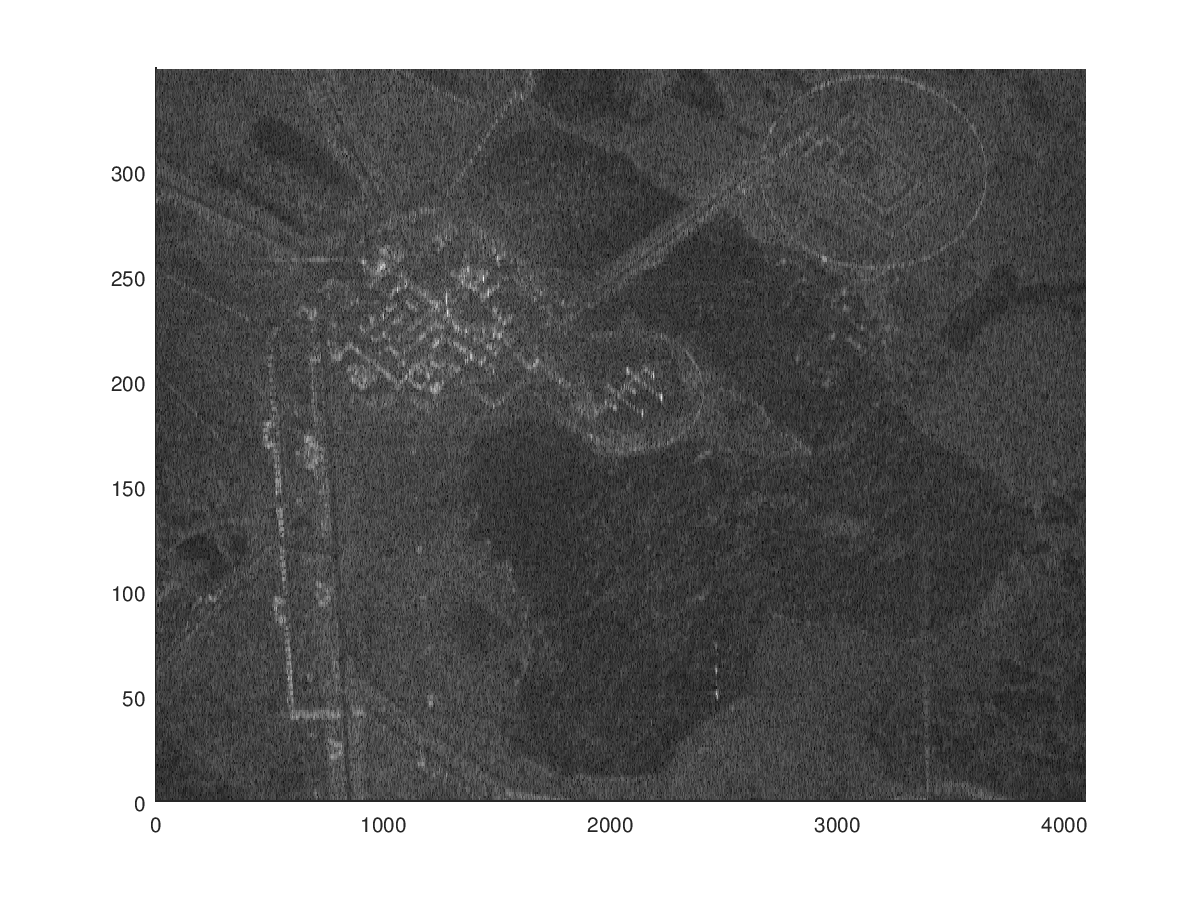
\includegraphics[width=\textwidth]{figures/task5.png}}}
  \caption{The filtered image.}
  \label{fig:task5_img}
\end{figure}
\begin{figure}[ht!]
  \centering
  \noindent\makebox[\textwidth]{\scalebox{0.90}{% Title: gl2ps_renderer figure
% Creator: GL2PS 1.3.9, (C) 1999-2015 C. Geuzaine
% For: Octave
% CreationDate: Fri May 26 21:01:21 2017
\setlength{\unitlength}{1pt}
\begin{picture}(0,0)
\includegraphics{figures/task5-inc.pdf}
\end{picture}%
\begin{picture}(576,432)(0,0)
\fontsize{10}{0}
\selectfont\put(74.88,42.5189){\makebox(0,0)[t]{\textcolor[rgb]{0.15,0.15,0.15}{{0}}}}
\fontsize{10}{0}
\selectfont\put(138.651,42.5189){\makebox(0,0)[t]{\textcolor[rgb]{0.15,0.15,0.15}{{50}}}}
\fontsize{10}{0}
\selectfont\put(202.423,42.5189){\makebox(0,0)[t]{\textcolor[rgb]{0.15,0.15,0.15}{{100}}}}
\fontsize{10}{0}
\selectfont\put(266.194,42.5189){\makebox(0,0)[t]{\textcolor[rgb]{0.15,0.15,0.15}{{150}}}}
\fontsize{10}{0}
\selectfont\put(329.966,42.5189){\makebox(0,0)[t]{\textcolor[rgb]{0.15,0.15,0.15}{{200}}}}
\fontsize{10}{0}
\selectfont\put(393.737,42.5189){\makebox(0,0)[t]{\textcolor[rgb]{0.15,0.15,0.15}{{250}}}}
\fontsize{10}{0}
\selectfont\put(457.509,42.5189){\makebox(0,0)[t]{\textcolor[rgb]{0.15,0.15,0.15}{{300}}}}
\fontsize{10}{0}
\selectfont\put(521.28,42.5189){\makebox(0,0)[t]{\textcolor[rgb]{0.15,0.15,0.15}{{350}}}}
\fontsize{10}{0}
\selectfont\put(69.8755,47.52){\makebox(0,0)[r]{\textcolor[rgb]{0.15,0.15,0.15}{{0}}}}
\fontsize{10}{0}
\selectfont\put(69.8755,97.8171){\makebox(0,0)[r]{\textcolor[rgb]{0.15,0.15,0.15}{{1e+09}}}}
\fontsize{10}{0}
\selectfont\put(69.8755,148.114){\makebox(0,0)[r]{\textcolor[rgb]{0.15,0.15,0.15}{{2e+09}}}}
\fontsize{10}{0}
\selectfont\put(69.8755,198.411){\makebox(0,0)[r]{\textcolor[rgb]{0.15,0.15,0.15}{{3e+09}}}}
\fontsize{10}{0}
\selectfont\put(69.8755,248.709){\makebox(0,0)[r]{\textcolor[rgb]{0.15,0.15,0.15}{{4e+09}}}}
\fontsize{10}{0}
\selectfont\put(69.8755,299.006){\makebox(0,0)[r]{\textcolor[rgb]{0.15,0.15,0.15}{{5e+09}}}}
\fontsize{10}{0}
\selectfont\put(69.8755,349.303){\makebox(0,0)[r]{\textcolor[rgb]{0.15,0.15,0.15}{{6e+09}}}}
\fontsize{10}{0}
\selectfont\put(69.8755,399.6){\makebox(0,0)[r]{\textcolor[rgb]{0.15,0.15,0.15}{{7e+09}}}}
\end{picture}
}}
  \caption{The squared magnitude of the filtered signal data.}
  \label{fig:task5_sig}
\end{figure}

\section{Task 6}
\subsection{a}
The pre-filtered power spectrum can be seen in Figure~\ref{fig:task6_pre} and the post-filtered power spectrum can be seen in Figure~\ref{fig:task6_post}. The Bandwidth is the same in both images but there post-filtered signal has been lowpass filtered.
\begin{figure}[ht!]
  \centering
    \begin{subfigure}[b]{0.59\textwidth}
        \noindent\makebox[\textwidth]{\scalebox{0.50}{% Title: gl2ps_renderer figure
% Creator: GL2PS 1.3.9, (C) 1999-2015 C. Geuzaine
% For: Octave
% CreationDate: Mon May 15 17:24:31 2017
\setlength{\unitlength}{1pt}
\begin{picture}(0,0)
\includegraphics{figures/task1-inc.pdf}
\end{picture}%
\begin{picture}(576,432)(0,0)
\fontsize{10}{0}
\selectfont\put(74.88,42.5189){\makebox(0,0)[t]{\textcolor[rgb]{0.15,0.15,0.15}{{-200}}}}
\fontsize{10}{0}
\selectfont\put(186.48,42.5189){\makebox(0,0)[t]{\textcolor[rgb]{0.15,0.15,0.15}{{-100}}}}
\fontsize{10}{0}
\selectfont\put(298.08,42.5189){\makebox(0,0)[t]{\textcolor[rgb]{0.15,0.15,0.15}{{0}}}}
\fontsize{10}{0}
\selectfont\put(409.68,42.5189){\makebox(0,0)[t]{\textcolor[rgb]{0.15,0.15,0.15}{{100}}}}
\fontsize{10}{0}
\selectfont\put(521.28,42.5189){\makebox(0,0)[t]{\textcolor[rgb]{0.15,0.15,0.15}{{200}}}}
\fontsize{10}{0}
\selectfont\put(69.8755,47.52){\makebox(0,0)[r]{\textcolor[rgb]{0.15,0.15,0.15}{{100000}}}}
\fontsize{10}{0}
\selectfont\put(69.8755,97.8171){\makebox(0,0)[r]{\textcolor[rgb]{0.15,0.15,0.15}{{150000}}}}
\fontsize{10}{0}
\selectfont\put(69.8755,148.114){\makebox(0,0)[r]{\textcolor[rgb]{0.15,0.15,0.15}{{200000}}}}
\fontsize{10}{0}
\selectfont\put(69.8755,198.411){\makebox(0,0)[r]{\textcolor[rgb]{0.15,0.15,0.15}{{250000}}}}
\fontsize{10}{0}
\selectfont\put(69.8755,248.709){\makebox(0,0)[r]{\textcolor[rgb]{0.15,0.15,0.15}{{300000}}}}
\fontsize{10}{0}
\selectfont\put(69.8755,299.006){\makebox(0,0)[r]{\textcolor[rgb]{0.15,0.15,0.15}{{350000}}}}
\fontsize{10}{0}
\selectfont\put(69.8755,349.303){\makebox(0,0)[r]{\textcolor[rgb]{0.15,0.15,0.15}{{400000}}}}
\fontsize{10}{0}
\selectfont\put(69.8755,399.6){\makebox(0,0)[r]{\textcolor[rgb]{0.15,0.15,0.15}{{450000}}}}
\fontsize{11}{0}
\selectfont\put(298.08,31.5188){\makebox(0,0)[t]{\textcolor[rgb]{0.15,0.15,0.15}{{Frequency (Hz)}}}}
\fontsize{11}{0}
\selectfont\put(29.8755,223.56){\rotatebox{90}{\makebox(0,0)[b]{\textcolor[rgb]{0.15,0.15,0.15}{{Power}}}}}
\fontsize{11}{0}
\selectfont\put(298.08,409.6){\makebox(0,0)[b]{\textcolor[rgb]{0,0,0}{{Power Spectral Density of azimuth spectrum}}}}
\end{picture}
}}
        \subcaption{Power spectrum pre-filtering.}
        \label{fig:task6_pre}
    \end{subfigure}\\
    \begin{subfigure}[b]{0.59\textwidth}
        \noindent\makebox[\textwidth]{\scalebox{0.50}{% Title: gl2ps_renderer figure
% Creator: GL2PS 1.3.9, (C) 1999-2015 C. Geuzaine
% For: Octave
% CreationDate: Fri May 26 21:29:49 2017
\setlength{\unitlength}{1pt}
\begin{picture}(0,0)
\includegraphics{figures/task6-inc.pdf}
\end{picture}%
\begin{picture}(576,432)(0,0)
\fontsize{10}{0}
\selectfont\put(74.88,42.5189){\makebox(0,0)[t]{\textcolor[rgb]{0.15,0.15,0.15}{{-200}}}}
\fontsize{10}{0}
\selectfont\put(186.48,42.5189){\makebox(0,0)[t]{\textcolor[rgb]{0.15,0.15,0.15}{{-100}}}}
\fontsize{10}{0}
\selectfont\put(298.08,42.5189){\makebox(0,0)[t]{\textcolor[rgb]{0.15,0.15,0.15}{{0}}}}
\fontsize{10}{0}
\selectfont\put(409.68,42.5189){\makebox(0,0)[t]{\textcolor[rgb]{0.15,0.15,0.15}{{100}}}}
\fontsize{10}{0}
\selectfont\put(521.28,42.5189){\makebox(0,0)[t]{\textcolor[rgb]{0.15,0.15,0.15}{{200}}}}
\fontsize{10}{0}
\selectfont\put(69.8755,47.52){\makebox(0,0)[r]{\textcolor[rgb]{0.15,0.15,0.15}{{0}}}}
\fontsize{10}{0}
\selectfont\put(69.8755,135.54){\makebox(0,0)[r]{\textcolor[rgb]{0.15,0.15,0.15}{{2e+08}}}}
\fontsize{10}{0}
\selectfont\put(69.8755,223.56){\makebox(0,0)[r]{\textcolor[rgb]{0.15,0.15,0.15}{{4e+08}}}}
\fontsize{10}{0}
\selectfont\put(69.8755,311.58){\makebox(0,0)[r]{\textcolor[rgb]{0.15,0.15,0.15}{{6e+08}}}}
\fontsize{10}{0}
\selectfont\put(69.8755,399.6){\makebox(0,0)[r]{\textcolor[rgb]{0.15,0.15,0.15}{{8e+08}}}}
\fontsize{11}{0}
\selectfont\put(298.08,31.5188){\makebox(0,0)[t]{\textcolor[rgb]{0.15,0.15,0.15}{{Frequency (Hz)}}}}
\fontsize{11}{0}
\selectfont\put(33.8755,223.56){\rotatebox{90}{\makebox(0,0)[b]{\textcolor[rgb]{0.15,0.15,0.15}{{Power}}}}}
\fontsize{11}{0}
\selectfont\put(298.08,409.6){\makebox(0,0)[b]{\textcolor[rgb]{0,0,0}{{Power Spectral Density of azimuth spectrum}}}}
\end{picture}
}}
        \subcaption{Power spectrum post-filtering.}
        \label{fig:task6_post}
    \end{subfigure}
  \caption{The pre- and post-filtered power spectrum for the signal data.}
  \label{fig:task6}
\end{figure}

\subsection{b}
The filter characteristics shown in Figure~\ref{fig:task6_filter} shows that the filter is a low-pass filter with an upper uniform frequency offset approximately 0.45, which corresponds to $\SI{140}{\hertz}$ (since 0.5 corresponds to 155 from \textit{spectrumplot}).
\begin{figure}[ht!]
  \centering
  \noindent\makebox[\textwidth]{\scalebox{0.90}{% Title: gl2ps_renderer figure
% Creator: GL2PS 1.3.9, (C) 1999-2015 C. Geuzaine
% For: Octave
% CreationDate: Fri May 26 22:05:07 2017
\setlength{\unitlength}{1pt}
\begin{picture}(0,0)
\includegraphics{figures/task6_filter-inc.pdf}
\end{picture}%
\begin{picture}(576,432)(0,0)
\fontsize{10}{0}
\selectfont\put(74.88,307.409){\makebox(0,0)[t]{\textcolor[rgb]{0.15,0.15,0.15}{{-0.8}}}}
\fontsize{10}{0}
\selectfont\put(130.68,307.409){\makebox(0,0)[t]{\textcolor[rgb]{0.15,0.15,0.15}{{-0.6}}}}
\fontsize{10}{0}
\selectfont\put(186.48,307.409){\makebox(0,0)[t]{\textcolor[rgb]{0.15,0.15,0.15}{{-0.4}}}}
\fontsize{10}{0}
\selectfont\put(242.28,307.409){\makebox(0,0)[t]{\textcolor[rgb]{0.15,0.15,0.15}{{-0.2}}}}
\fontsize{10}{0}
\selectfont\put(298.08,307.409){\makebox(0,0)[t]{\textcolor[rgb]{0.15,0.15,0.15}{{0}}}}
\fontsize{10}{0}
\selectfont\put(353.88,307.409){\makebox(0,0)[t]{\textcolor[rgb]{0.15,0.15,0.15}{{0.2}}}}
\fontsize{10}{0}
\selectfont\put(409.68,307.409){\makebox(0,0)[t]{\textcolor[rgb]{0.15,0.15,0.15}{{0.4}}}}
\fontsize{10}{0}
\selectfont\put(465.48,307.409){\makebox(0,0)[t]{\textcolor[rgb]{0.15,0.15,0.15}{{0.6}}}}
\fontsize{10}{0}
\selectfont\put(521.28,307.409){\makebox(0,0)[t]{\textcolor[rgb]{0.15,0.15,0.15}{{0.8}}}}
\fontsize{10}{0}
\selectfont\put(69.8755,312.433){\makebox(0,0)[r]{\textcolor[rgb]{0.15,0.15,0.15}{{15}}}}
\fontsize{10}{0}
\selectfont\put(69.8755,333.786){\makebox(0,0)[r]{\textcolor[rgb]{0.15,0.15,0.15}{{20}}}}
\fontsize{10}{0}
\selectfont\put(69.8755,355.139){\makebox(0,0)[r]{\textcolor[rgb]{0.15,0.15,0.15}{{25}}}}
\fontsize{10}{0}
\selectfont\put(69.8755,376.492){\makebox(0,0)[r]{\textcolor[rgb]{0.15,0.15,0.15}{{30}}}}
\fontsize{10}{0}
\selectfont\put(69.8755,397.845){\makebox(0,0)[r]{\textcolor[rgb]{0.15,0.15,0.15}{{35}}}}
\fontsize{11}{0}
\selectfont\put(298.08,296.409){\makebox(0,0)[t]{\textcolor[rgb]{0.15,0.15,0.15}{{Uniform frequency}}}}
\fontsize{11}{0}
\selectfont\put(53.8755,355.139){\rotatebox{90}{\makebox(0,0)[b]{\textcolor[rgb]{0.15,0.15,0.15}{{Power (dB)}}}}}
\fontsize{11}{0}
\selectfont\put(298.08,407.845){\makebox(0,0)[b]{\textcolor[rgb]{0,0,0}{{Filter properties}}}}
\fontsize{10}{0}
\selectfont\put(119.52,174.952){\makebox(0,0)[t]{\textcolor[rgb]{0.15,0.15,0.15}{{-0.4}}}}
\fontsize{10}{0}
\selectfont\put(208.8,174.952){\makebox(0,0)[t]{\textcolor[rgb]{0.15,0.15,0.15}{{-0.2}}}}
\fontsize{10}{0}
\selectfont\put(298.08,174.952){\makebox(0,0)[t]{\textcolor[rgb]{0.15,0.15,0.15}{{0}}}}
\fontsize{10}{0}
\selectfont\put(387.36,174.952){\makebox(0,0)[t]{\textcolor[rgb]{0.15,0.15,0.15}{{0.2}}}}
\fontsize{10}{0}
\selectfont\put(476.64,174.952){\makebox(0,0)[t]{\textcolor[rgb]{0.15,0.15,0.15}{{0.4}}}}
\fontsize{10}{0}
\selectfont\put(69.8755,181.152){\makebox(0,0)[r]{\textcolor[rgb]{0.15,0.15,0.15}{{-1000}}}}
\fontsize{10}{0}
\selectfont\put(69.8755,197.999){\makebox(0,0)[r]{\textcolor[rgb]{0.15,0.15,0.15}{{-800}}}}
\fontsize{10}{0}
\selectfont\put(69.8755,214.846){\makebox(0,0)[r]{\textcolor[rgb]{0.15,0.15,0.15}{{-600}}}}
\fontsize{10}{0}
\selectfont\put(69.8755,231.694){\makebox(0,0)[r]{\textcolor[rgb]{0.15,0.15,0.15}{{-400}}}}
\fontsize{10}{0}
\selectfont\put(69.8755,248.541){\makebox(0,0)[r]{\textcolor[rgb]{0.15,0.15,0.15}{{-200}}}}
\fontsize{10}{0}
\selectfont\put(69.8755,265.388){\makebox(0,0)[r]{\textcolor[rgb]{0.15,0.15,0.15}{{0}}}}
\fontsize{11}{0}
\selectfont\put(298.08,163.952){\makebox(0,0)[t]{\textcolor[rgb]{0.15,0.15,0.15}{{Uniform frequency}}}}
\fontsize{11}{0}
\selectfont\put(37.8755,222.682){\rotatebox{90}{\makebox(0,0)[b]{\textcolor[rgb]{0.15,0.15,0.15}{{Angle (rad)}}}}}
\fontsize{10}{0}
\selectfont\put(119.52,42.4958){\makebox(0,0)[t]{\textcolor[rgb]{0.15,0.15,0.15}{{-0.4}}}}
\fontsize{10}{0}
\selectfont\put(208.8,42.4958){\makebox(0,0)[t]{\textcolor[rgb]{0.15,0.15,0.15}{{-0.2}}}}
\fontsize{10}{0}
\selectfont\put(298.08,42.4958){\makebox(0,0)[t]{\textcolor[rgb]{0.15,0.15,0.15}{{0}}}}
\fontsize{10}{0}
\selectfont\put(387.36,42.4958){\makebox(0,0)[t]{\textcolor[rgb]{0.15,0.15,0.15}{{0.2}}}}
\fontsize{10}{0}
\selectfont\put(476.64,42.4958){\makebox(0,0)[t]{\textcolor[rgb]{0.15,0.15,0.15}{{0.4}}}}
\fontsize{10}{0}
\selectfont\put(69.8755,56.0612){\makebox(0,0)[r]{\textcolor[rgb]{0.15,0.15,0.15}{{-400}}}}
\fontsize{10}{0}
\selectfont\put(69.8755,73.1435){\makebox(0,0)[r]{\textcolor[rgb]{0.15,0.15,0.15}{{-200}}}}
\fontsize{10}{0}
\selectfont\put(69.8755,90.2259){\makebox(0,0)[r]{\textcolor[rgb]{0.15,0.15,0.15}{{0}}}}
\fontsize{10}{0}
\selectfont\put(69.8755,107.308){\makebox(0,0)[r]{\textcolor[rgb]{0.15,0.15,0.15}{{200}}}}
\fontsize{10}{0}
\selectfont\put(69.8755,124.391){\makebox(0,0)[r]{\textcolor[rgb]{0.15,0.15,0.15}{{400}}}}
\fontsize{11}{0}
\selectfont\put(298.08,31.4958){\makebox(0,0)[t]{\textcolor[rgb]{0.15,0.15,0.15}{{Uniform frequency}}}}
\fontsize{11}{0}
\selectfont\put(43.8755,90.2259){\rotatebox{90}{\makebox(0,0)[b]{\textcolor[rgb]{0.15,0.15,0.15}{{Group delay}}}}}
\end{picture}
}}
  \caption{Filter characteristics.}
  \label{fig:task6_filter}
\end{figure}

The signal spreads in time but is constant in frequency as it propagates, so the higher resolution likely comes from reconstructing the original signal in time using the filter.

\section{Task 7}
There nine-look filtered image can be seen in Figure~\ref{fig:task7_nlf}. The image now looks a lost clearer compared to Figure~\ref{fig:task7_f}.

The bandwidth of the peak seen in Figure~\ref{fig:task7_ps} is now about 9 points wide which means that the resolution has decreased to $9\Delta A=\SI{3.9}{\metre}$. The pixel size is unaffected by the multi-looking process.
\begin{figure}[ht!]
  \centering
    \begin{subfigure}[b]{0.59\textwidth}
        \noindent\makebox[\textwidth]{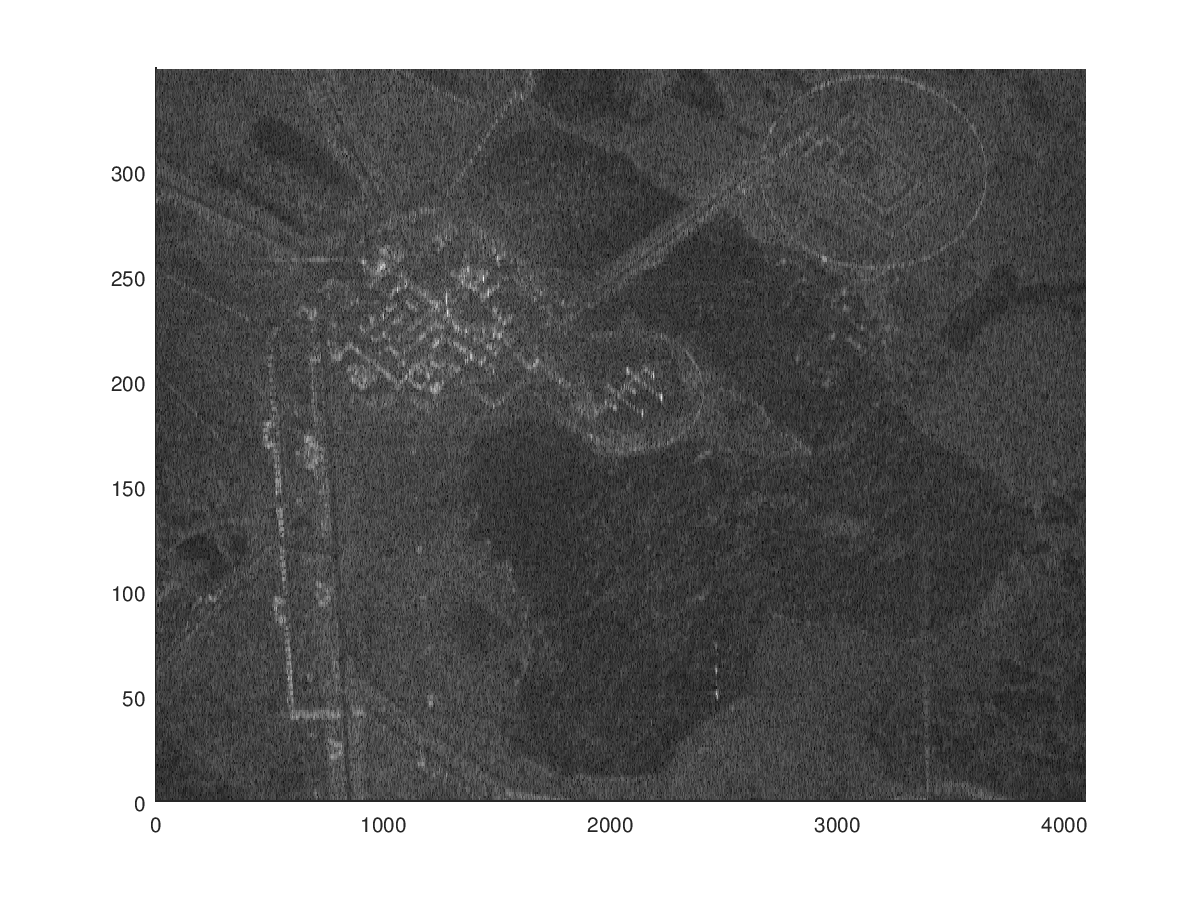
\includegraphics[width=\textwidth]{figures/task5.png}}
        \subcaption{The filtered image.}
        \label{fig:task7_f}
    \end{subfigure}\\
    \begin{subfigure}[b]{0.59\textwidth}
        \noindent\makebox[\textwidth]{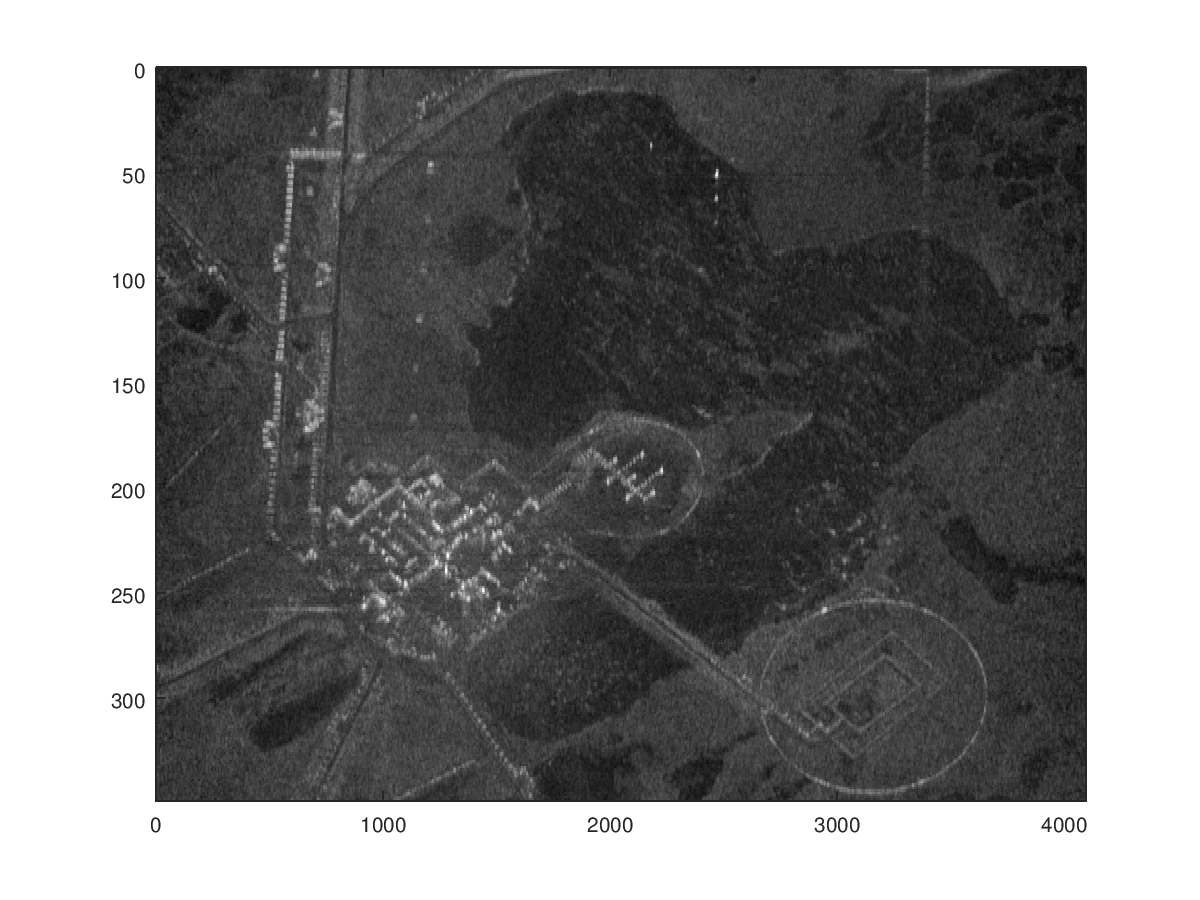
\includegraphics[width=\textwidth]{figures/task7.png}}
        \subcaption{The nine-look filtered image.}
        \label{fig:task7_nlf}
    \end{subfigure}
  \caption{The images before and after nine-look.}
  \label{fig:task7_img}
\end{figure}
\begin{figure}[ht!]
  \centering
    \begin{subfigure}[b]{0.59\textwidth}
        \noindent\makebox[\textwidth]{\scalebox{0.50}{% Title: gl2ps_renderer figure
% Creator: GL2PS 1.3.9, (C) 1999-2015 C. Geuzaine
% For: Octave
% CreationDate: Fri May 26 23:37:58 2017
\setlength{\unitlength}{1pt}
\begin{picture}(0,0)
\includegraphics{figures/task7_spct1-inc.pdf}
\end{picture}%
\begin{picture}(576,432)(0,0)
\fontsize{10}{0}
\selectfont\put(74.88,42.5189){\makebox(0,0)[t]{\textcolor[rgb]{0.15,0.15,0.15}{{0}}}}
\fontsize{10}{0}
\selectfont\put(164.16,42.5189){\makebox(0,0)[t]{\textcolor[rgb]{0.15,0.15,0.15}{{1000}}}}
\fontsize{10}{0}
\selectfont\put(253.44,42.5189){\makebox(0,0)[t]{\textcolor[rgb]{0.15,0.15,0.15}{{2000}}}}
\fontsize{10}{0}
\selectfont\put(342.72,42.5189){\makebox(0,0)[t]{\textcolor[rgb]{0.15,0.15,0.15}{{3000}}}}
\fontsize{10}{0}
\selectfont\put(432,42.5189){\makebox(0,0)[t]{\textcolor[rgb]{0.15,0.15,0.15}{{4000}}}}
\fontsize{10}{0}
\selectfont\put(521.28,42.5189){\makebox(0,0)[t]{\textcolor[rgb]{0.15,0.15,0.15}{{5000}}}}
\fontsize{10}{0}
\selectfont\put(69.8755,47.52){\makebox(0,0)[r]{\textcolor[rgb]{0.15,0.15,0.15}{{0}}}}
\fontsize{10}{0}
\selectfont\put(69.8755,106.2){\makebox(0,0)[r]{\textcolor[rgb]{0.15,0.15,0.15}{{2e+07}}}}
\fontsize{10}{0}
\selectfont\put(69.8755,164.88){\makebox(0,0)[r]{\textcolor[rgb]{0.15,0.15,0.15}{{4e+07}}}}
\fontsize{10}{0}
\selectfont\put(69.8755,223.56){\makebox(0,0)[r]{\textcolor[rgb]{0.15,0.15,0.15}{{6e+07}}}}
\fontsize{10}{0}
\selectfont\put(69.8755,282.24){\makebox(0,0)[r]{\textcolor[rgb]{0.15,0.15,0.15}{{8e+07}}}}
\fontsize{10}{0}
\selectfont\put(69.8755,340.92){\makebox(0,0)[r]{\textcolor[rgb]{0.15,0.15,0.15}{{1e+08}}}}
\fontsize{10}{0}
\selectfont\put(69.8755,399.6){\makebox(0,0)[r]{\textcolor[rgb]{0.15,0.15,0.15}{{1.2e+08}}}}
\end{picture}
}}
        \subcaption{Power spectrum of nine-look image}
        \label{fig:task7_ps_whole}
    \end{subfigure}\\
    \begin{subfigure}[b]{0.59\textwidth}
        \noindent\makebox[\textwidth]{\scalebox{0.50}{% Title: gl2ps_renderer figure
% Creator: GL2PS 1.3.9, (C) 1999-2015 C. Geuzaine
% For: Octave
% CreationDate: Fri May 26 23:40:49 2017
\setlength{\unitlength}{1pt}
\begin{picture}(0,0)
\includegraphics{figures/task7_spct2-inc.pdf}
\end{picture}%
\begin{picture}(576,432)(0,0)
\fontsize{10}{0}
\selectfont\put(174.211,42.5189){\makebox(0,0)[t]{\textcolor[rgb]{0.15,0.15,0.15}{{2170}}}}
\fontsize{10}{0}
\selectfont\put(293.646,42.5189){\makebox(0,0)[t]{\textcolor[rgb]{0.15,0.15,0.15}{{2180}}}}
\fontsize{10}{0}
\selectfont\put(413.081,42.5189){\makebox(0,0)[t]{\textcolor[rgb]{0.15,0.15,0.15}{{2190}}}}
\fontsize{10}{0}
\selectfont\put(69.8752,52.2811){\makebox(0,0)[r]{\textcolor[rgb]{0.15,0.15,0.15}{{0}}}}
\fontsize{10}{0}
\selectfont\put(69.8752,114.13){\makebox(0,0)[r]{\textcolor[rgb]{0.15,0.15,0.15}{{2e+07}}}}
\fontsize{10}{0}
\selectfont\put(69.8752,175.979){\makebox(0,0)[r]{\textcolor[rgb]{0.15,0.15,0.15}{{4e+07}}}}
\fontsize{10}{0}
\selectfont\put(69.8752,237.828){\makebox(0,0)[r]{\textcolor[rgb]{0.15,0.15,0.15}{{6e+07}}}}
\fontsize{10}{0}
\selectfont\put(69.8752,299.677){\makebox(0,0)[r]{\textcolor[rgb]{0.15,0.15,0.15}{{8e+07}}}}
\fontsize{10}{0}
\selectfont\put(69.8752,361.526){\makebox(0,0)[r]{\textcolor[rgb]{0.15,0.15,0.15}{{1e+08}}}}
\end{picture}
}}
        \subcaption{Power spectrum of nine-look image close to its peak.}
        \label{fig:task7_ps_zoom}
    \end{subfigure}
  \caption{The power spectrum of the nine-look image (same row as \textit{oneline})}
  \label{fig:task7_ps}
\end{figure}


\newpage
\appendix
\section{Code}
\subsection{Task 1}
\begin{changemargin}{-3cm}{0.5cm}
\lstinputlisting[language=MATLAB]{task1.m}
\end{changemargin}
\subsection{Task 2}
\begin{changemargin}{-3cm}{0.5cm}
\lstinputlisting[language=MATLAB]{task2.m}
\end{changemargin}
\subsection{Task 3}
\begin{changemargin}{-3cm}{0.5cm}
\lstinputlisting[language=MATLAB]{task3.m}
\end{changemargin}
\subsection{Task 4}
\begin{changemargin}{-3cm}{0.5cm}
\lstinputlisting[language=MATLAB]{task4.m}
\end{changemargin}
\subsection{Task 5}
\begin{changemargin}{-3cm}{0.5cm}
\lstinputlisting[language=MATLAB]{task5.m}
\end{changemargin}
\subsection{Task 6}
\begin{changemargin}{-3cm}{0.5cm}
\lstinputlisting[language=MATLAB]{task6.m}
\end{changemargin}
\subsection{Task 7}
\begin{changemargin}{-3cm}{0.5cm}
\lstinputlisting[language=MATLAB]{task7.m}
\end{changemargin}

\end{document}